\documentclass[10pt,a4paper]{article}
\usepackage[margin=0.52in]{geometry}
\usepackage{graphicx}
\usepackage{booktabs}
\usepackage{float}
\usepackage{enumitem}
\usepackage{url}
\usepackage[hidelinks]{hyperref}
\setlist{nosep,leftmargin=*,topsep=2pt}
\urlstyle{same}
\setlength{\parskip}{0.2em}

\title{\textbf{Task 1: LoRA Rank Ablation Study with MLX-LM}}
\author{TinyLlama Instruction Tuning Project}
\date{\today}

\begin{document}
\maketitle
\vspace{-1em}

\section*{Task description}
{\small
We study how LoRA rank affects cost and quality on Apple Silicon: train \textbf{five} TinyLlama models with ranks $4,8,16,32,64$ and fixed $\alpha/r=2$. For each run we record \textbf{wall-clock training time}, \textbf{peak Metal memory}, \textbf{final test loss}, and \textbf{inference latency} (ms/token, tok/s) over \textbf{100} Alpaca-format test prompts. We fill a comparison matrix with rank, throughput, memory, and \textbf{MMLU-style} accuracy (4-option MCQ), identify the \textbf{Pareto-optimal} rank using \textbf{accuracy vs.\ latency} only, and save matplotlib \texttt{.png} plots for reporting.
}

\section*{Procedure \& technical implementation}
{\small
\begin{enumerate}[label=\textbf{\arabic*.}]
  \item \textbf{Environment.} Python~3, MLX / \texttt{mlx-lm}; Apple Silicon with Metal. Entry point: \path{task1_lora_rank_ablation.py} (also \texttt{make task1}).
  \item \textbf{LoRA configs.} Base model \texttt{TinyLlama/TinyLlama-1.1B-Chat-v1.0}; training data path \path{./data/}; LoRA modules \texttt{self\_attn.q\_proj}, \texttt{self\_attn.v\_proj}; rank $r$; $\alpha=2r$, \texttt{scale}$=\alpha/r=2$; batch~2; default 2000 iterations; LR $2{\times}10^{-4}$; YAML per rank under \path{results/task1/}.
  \item \textbf{Metrics from training.} Subprocess isolation for fair peak memory; regex parse of test loss from \texttt{mlx\_lm} logs; \texttt{train\_time\_sec} wall clock.
  \item \textbf{Inference benchmark.} Load base + adapter; read first 100 user messages from \path{data/test.jsonl}; warm-up; generate up to 100 tokens each; compute global ms/token and tok/s.
  \item \textbf{MMLU-style accuracy.} \path{evaluate_mmlu_accuracy.py}: for each of 100 test rows, build one MCQ with the gold answer plus three distractors from other rows; model must reply with A/B/C/D; accuracy $=$ fraction correct $\times 100$. Stored in the comparison matrix and \path{accuracy_results.json}.
  \item \textbf{Pareto (2D).} Frontier: maximize MCQ accuracy, minimize \texttt{ms\_per\_token}; memory \emph{excluded}. Among non-dominated points, select rank with $0.5$ normalized accuracy $+$ $0.5$ normalized latency. Artifacts: \path{comparison_matrix.json}, \path{pareto.json}, \path{rank_ablation_metrics.png}, \path{memory_speed_curves.png}, \path{pareto_analysis.png}.
\end{enumerate}
}

\section*{Results}
{\small
\textbf{Quantitative summary.} Table~\ref{tab:t1} uses values from \path{results/task1/comparison_matrix.json} (training times converted to minutes). MCQ columns in JSON may be zero until \path{evaluate_mmlu_accuracy.py} is run after the MCQ update---re-run the task script to populate. Current 2D Pareto choice: rank~\textbf{8} (\path{pareto.json}). Ranks~8--16 achieve the best test loss in this run; rank~8 leads in tok/s.
\begin{table}[H]
\centering
\caption{LoRA rank ablation (checked-in \texttt{comparison\_matrix.json}).}
\label{tab:t1}
\footnotesize
\begin{tabular}{@{}rcccccc@{}}
\toprule
$r$ & Time (min) & Mem (MB) & Test loss & tok/s & ms/tok & MCQ \% \\
\midrule
4  & 19.3 & 3057 & 1.263 & 96.8 & 10.33 & 22.0 \\
8  & 18.9 & 3066 & 1.262 & 99.1 & 10.09 & 19.0 \\
16 & 18.7 & 3075 & 1.262 & 98.9 & 10.12 & 17.0 \\
32 & 19.2 & 3100 & 1.265 & 97.5 & 10.26 & 17.0 \\
64 & 19.5 & 3151 & 1.270 & 95.7 & 10.45 & 18.0 \\
\bottomrule
\end{tabular}\\[3pt]
\scriptsize MCQ \% values shown here are from \path{results/task1/accuracy_results.json}; re-run \path{evaluate_mmlu_accuracy.py} to refresh after new checkpoints.
\end{table}
}

\section*{Evidence (screenshots)}
{\small
\textbf{Figure~\ref{fig:t1}} is a matplotlib export saved by the pipeline: three panels (peak memory, inference speed, test loss vs.\ rank). Running the script also writes \path{memory_speed_curves.png} and \path{pareto_analysis.png} (accuracy--latency scatter with frontier); add those files to \path{results/task1/} for the full figure set.
\begin{figure}[H]
\centering
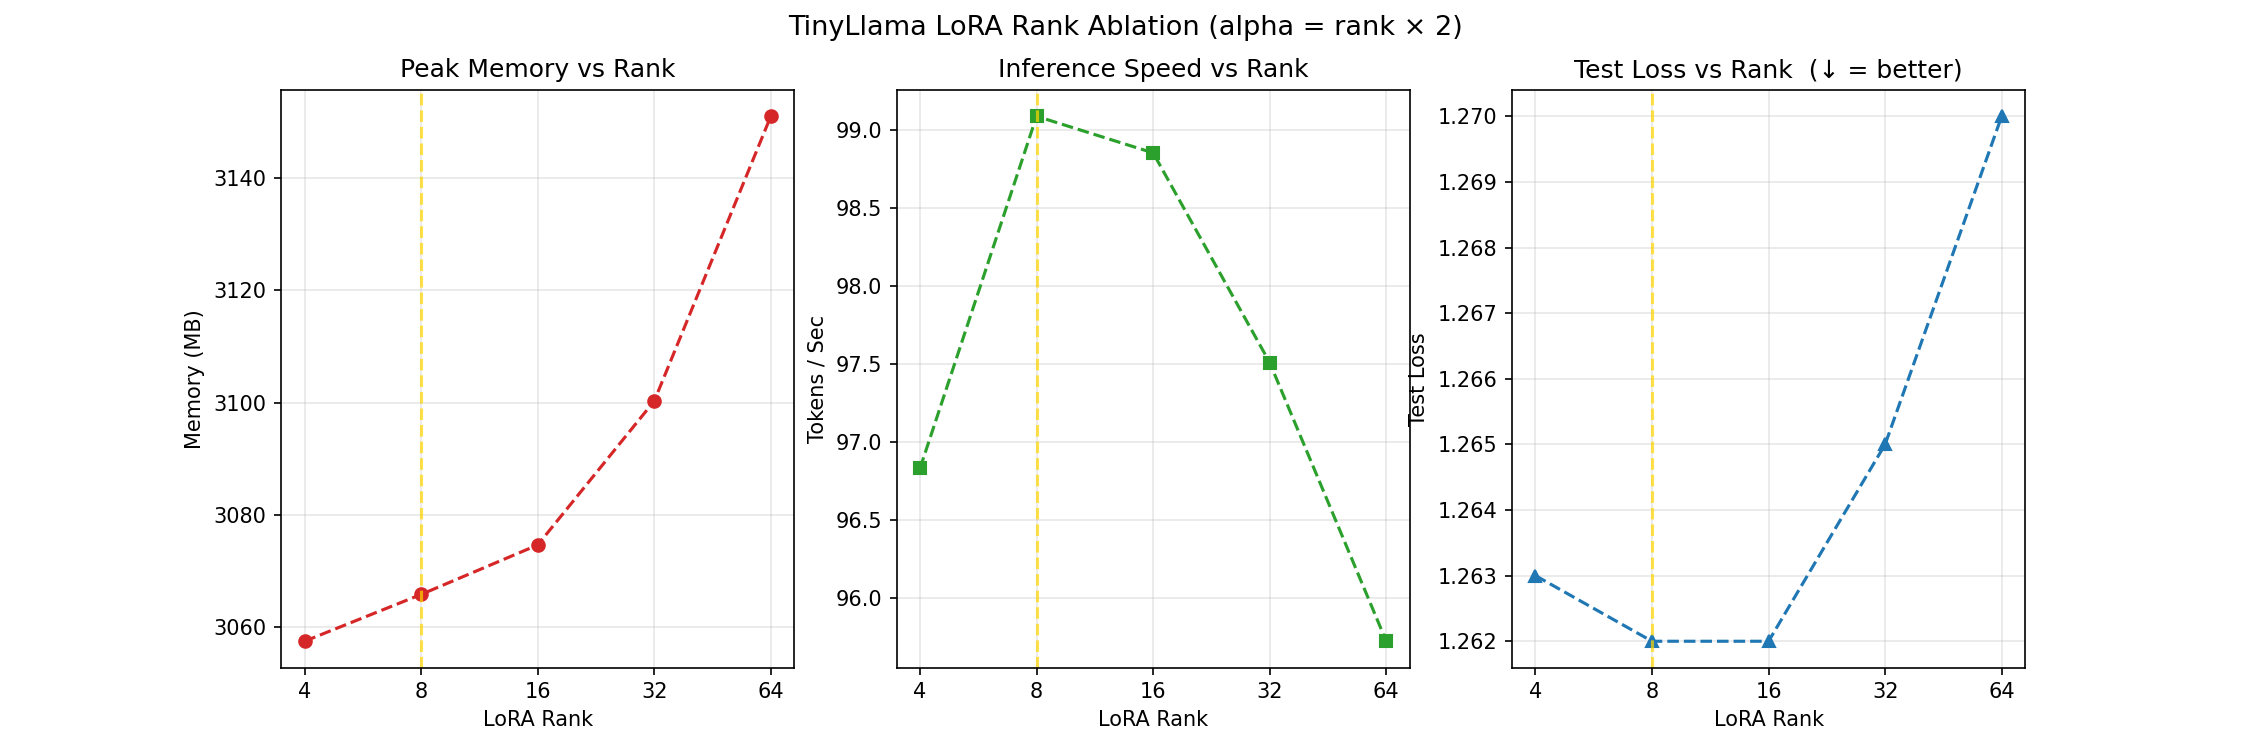
\includegraphics[width=0.92\linewidth]{../results/task1/rank_ablation_metrics.png}
\caption{Task~1 visualization: memory (left), throughput (center), test loss (right) vs.\ LoRA rank. Regenerate with \texttt{make task1}.}
\label{fig:t1}
\end{figure}
}

\end{document}
